\documentclass[border=10pt]{standalone}
\usepackage{tikz}
\usetikzlibrary{arrows.meta,calc}

\begin{document}
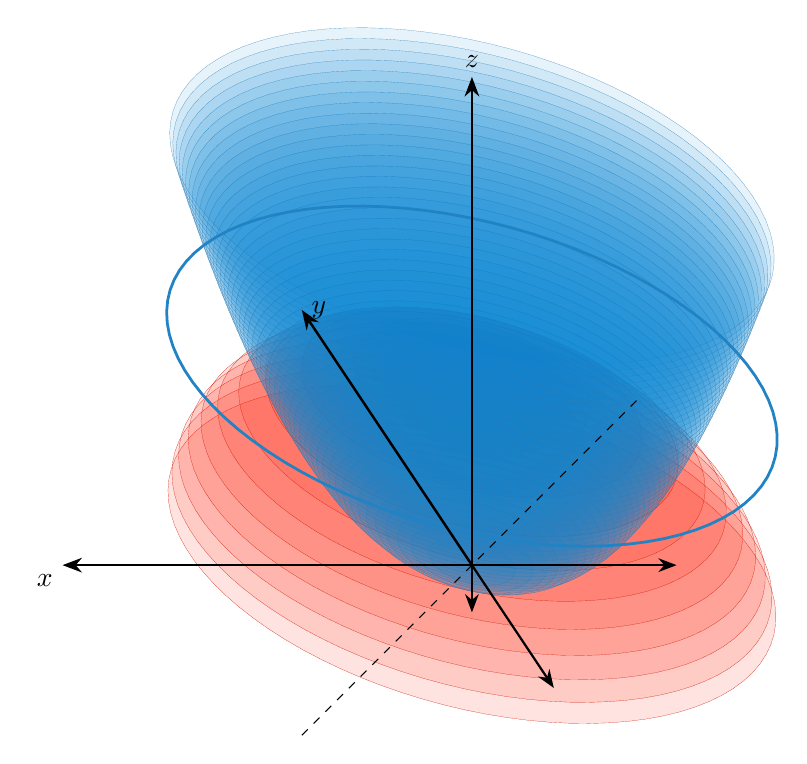
\begin{tikzpicture}[scale=2,
    >=Stealth,
    line join=round,
    x={(1cm,0cm)},
    y={(-0.4cm,0.6cm)},
    z={(0cm,1cm)}
]

% Parameters
\def\R{1.8}     % radius of intersection circle
\def\H{2.4}     % height of top of blue surface
\def\Hb{1.2}    % height of pink cap
\def\steps{45}  % radial sampling for meshes

% Colors
\colorlet{blueSurf}{cyan!70!blue}
\colorlet{pinkSurf}{orange!20!red}

%%%%%%%%%%%%%%%%%%%%%%%%%%%%%%%%%%%%%%%%%%%%%%%%%%%%%%%%%%%%
% Helper macro: circle (or ellipse) in xy-plane at given z
%%%%%%%%%%%%%%%%%%%%%%%%%%%%%%%%%%%%%%%%%%%%%%%%%%%%%%%%%%%%
\newcommand{\horizcircle}[3][]{%
    % #1 options, #2 radius in xy-plane, #3 height (z)
    \draw[#1,domain=0:360,samples=90,variable=\t]
        plot ({#2*cos(\t)},{#2*sin(\t)},{#3});
}

%%%%%%%%%%%%%%%%%%%%%%%%%%%%%%%%%%%%%%%%%%%%%%%%%%%%%%%%%%%%
% Pink lower surface (downward-looking cap)
% Represented as many low-opacity horizontal circles
%%%%%%%%%%%%%%%%%%%%%%%%%%%%%%%%%%%%%%%%%%%%%%%%%%%%%%%%%%%%
\foreach \k in {0.1,0.2,...,1.0} {
    % radius and height relationship to mimic a dome-like bowl
    \pgfmathsetmacro{\rr}{\R*sqrt(1 - 0.85*(\k)^2)}
    \pgfmathsetmacro{\zz}{\Hb*\k}
    \horizcircle[draw=pinkSurf!80!black, line width=0.06pt,
                 fill=pinkSurf, fill opacity=0.12]{\rr}{\zz-0.05}
}

%%%%%%%%%%%%%%%%%%%%%%%%%%%%%%%%%%%%%%%%%%%%%%%%%%%%%%%%%%%%
% Blue upper surface (paraboloid-like funnel)
% Many horizontal circles increasing with z
%%%%%%%%%%%%%%%%%%%%%%%%%%%%%%%%%%%%%%%%%%%%%%%%%%%%%%%%%%%%
\foreach \k in {0.0,0.02,...,1.0} {
    % radius as function of height: narrow at origin, larger near rim
    \pgfmathsetmacro{\zz}{\H*(\k)^1.2}
    \pgfmathsetmacro{\rr}{\R*sqrt(\k)};
    \horizcircle[draw=blueSurf!80!black, line width=0.05pt,
                 fill=blueSurf, fill opacity=0.10]{\rr}{\zz}
}

% Intersection circle (rim) stronger
\horizcircle[draw=blueSurf!90!black, line width=1.0pt]{\R}{\Hb}

%%%%%%%%%%%%%%%%%%%%%%%%%%%%%%%%%%%%%%%%%%%%%%%%%%%%%%%%%%%%
% Axes
%%%%%%%%%%%%%%%%%%%%%%%%%%%%%%%%%%%%%%%%%%%%%%%%%%%%%%%%%%%%

% Origin
\coordinate (O) at (0,0,0);

% Axis endpoints (in xyz coordinates)
\coordinate (X) at (-2.6,0,0);
\coordinate (Xm) at (1.3,0,0);
\coordinate (Y) at (0,2.7,0);
\coordinate (Ym) at (0,-1.3,0);
\coordinate (Z) at (0,0,3.1);
\coordinate (Zm) at (0,0,-0.3);

% Draw axes: first back parts
\draw[->,line width=0.8pt] (O) -- (Xm);
\draw[->,line width=0.8pt] (O) -- (Ym);
\draw[->,line width=0.8pt] (O) -- (Zm);

% Front parts
\draw[->,line width=0.9pt] (O) -- (X);
\draw[->,line width=0.9pt] (O) -- (Y);
\draw[->,line width=0.9pt] (O) -- (Z);

% Axis labels
\node[anchor=north east] at (X) {$x$};
\node[anchor=west]       at (Y) {$y$};
\node[anchor=south]      at (Z) {$z$};

%%%%%%%%%%%%%%%%%%%%%%%%%%%%%%%%%%%%%%%%%%%%%%%%%%%%%%%%%%%%
% Dashed diagonal in base plane (indicating hidden axis)
%%%%%%%%%%%%%%%%%%%%%%%%%%%%%%%%%%%%%%%%%%%%%%%%%%%%%%%%%%%%
\draw[dashed, line width=0.4pt]
    (-1.8,-1.8,0) -- (1.8,1.8,0);

\end{tikzpicture}
\end{document}